\documentclass{standalone}
\usepackage{tikz}
\usetikzlibrary{patterns, positioning}
\usepackage[sfdefault]{ClearSans} %% option 'sfdefault' activates Clear Sans as the default text font
\usepackage[T1]{fontenc}

\begin{document}
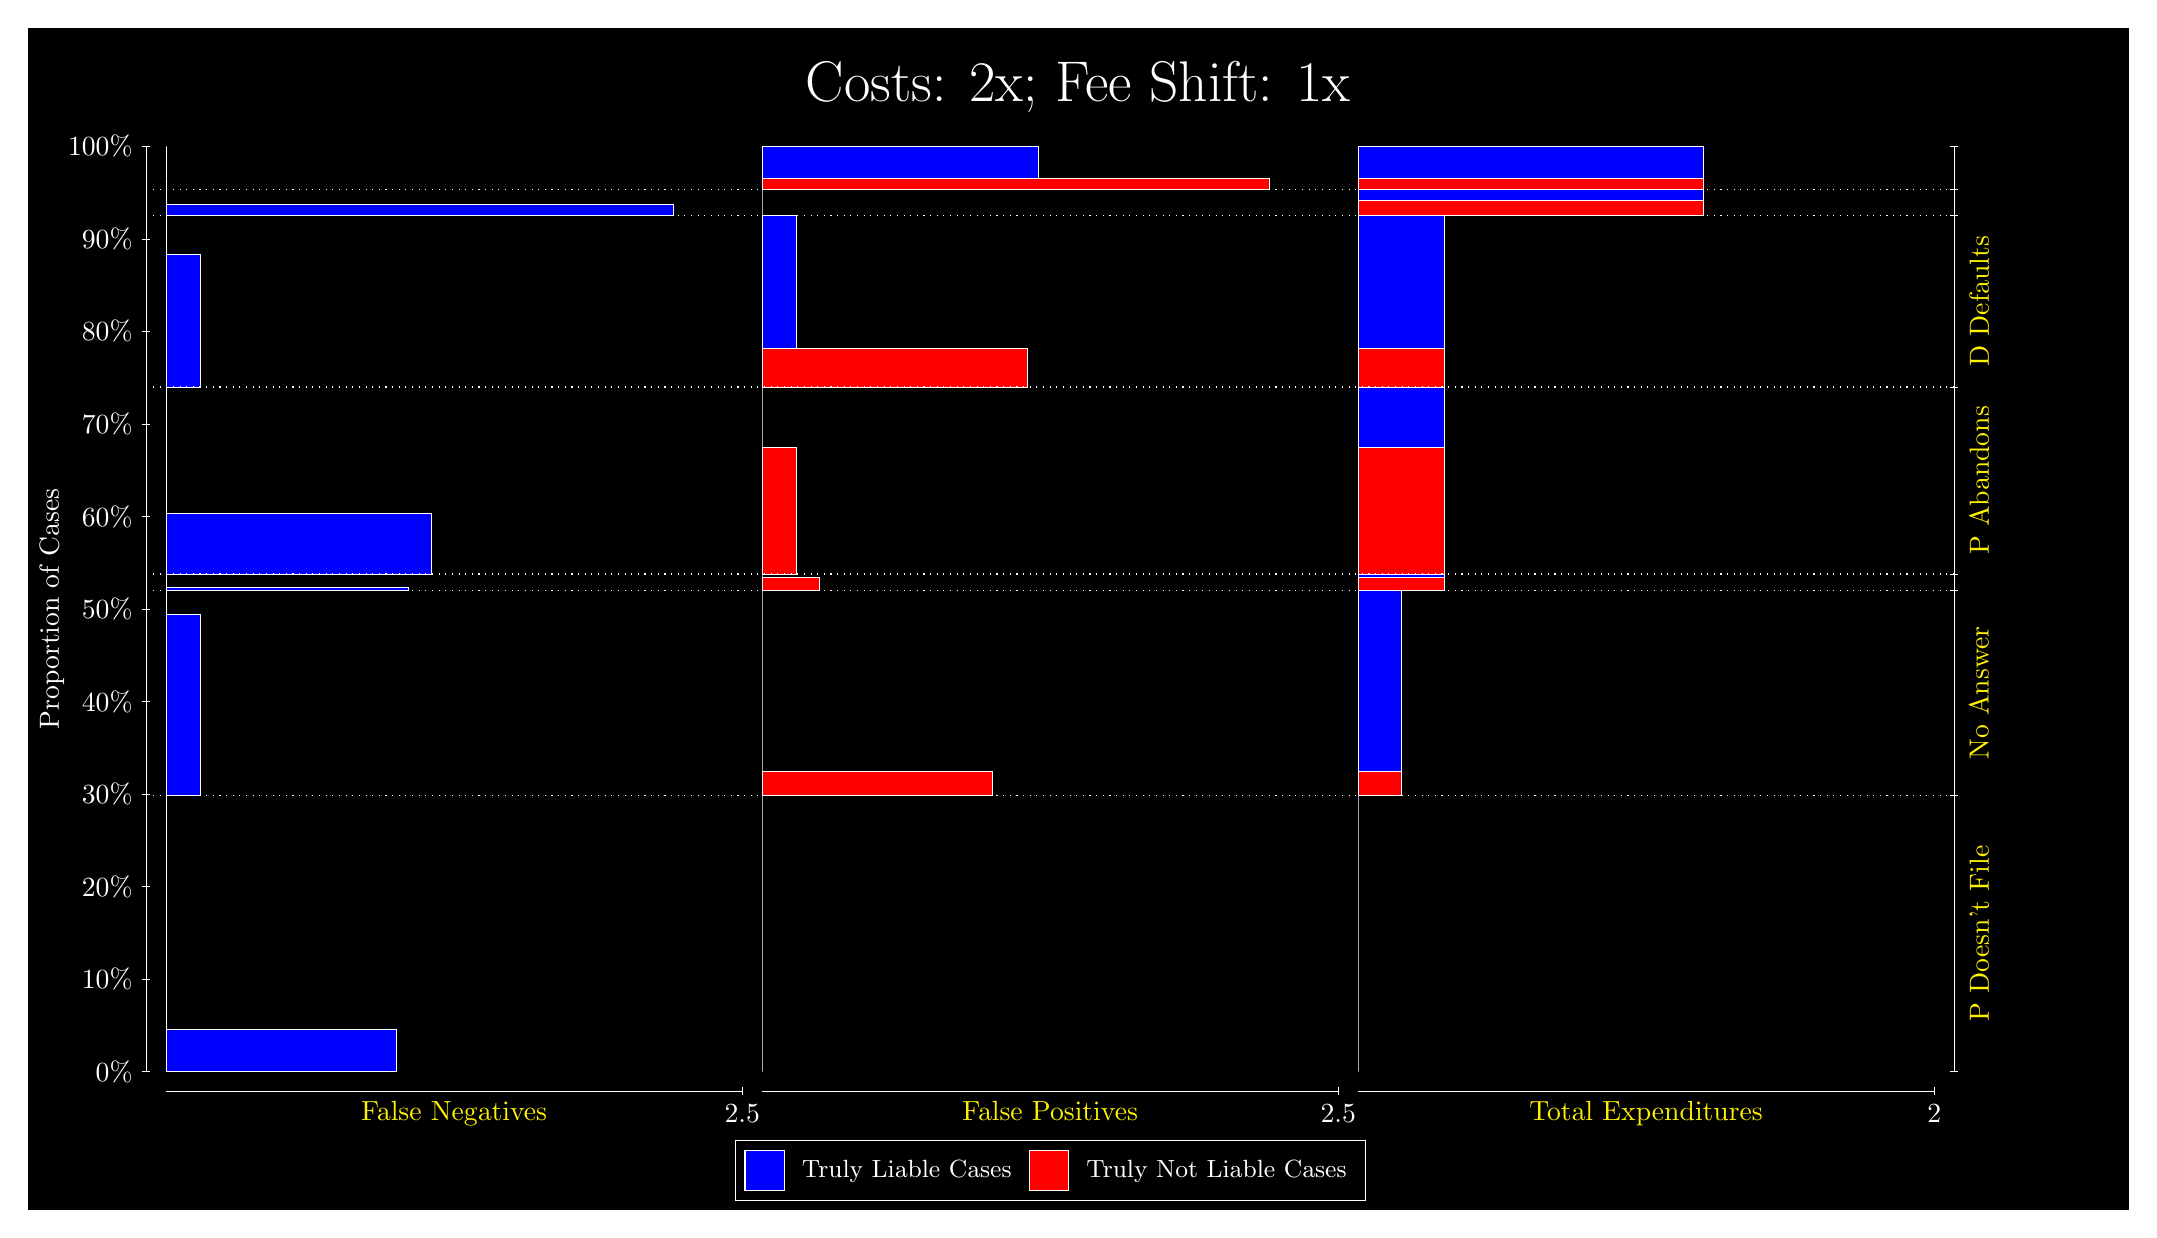
\begin{tikzpicture}
\draw[fill=black] (0,0) rectangle (26.667,15);
\draw[text=white] (0,13.5) rectangle (26.667,15) node[midway] {\huge Costs: 2x; Fee Shift: 1x};
\draw[white, very thin] (1.5,1.75) -- (1.5,13.5);
\node[rotate=90, text=white, anchor=center] at (0.3, 7.625) {Proportion of Cases};
\draw[white, very thin] (1.45,1.75) -- (1.55,1.75);
\node[text=white, anchor=east] at (1.45, 1.75) {0\%};
\draw[white, very thin] (1.45,2.925) -- (1.55,2.925);
\node[text=white, anchor=east] at (1.45, 2.925) {10\%};
\draw[white, very thin] (1.45,4.1) -- (1.55,4.1);
\node[text=white, anchor=east] at (1.45, 4.1) {20\%};
\draw[white, very thin] (1.45,5.275) -- (1.55,5.275);
\node[text=white, anchor=east] at (1.45, 5.275) {30\%};
\draw[white, very thin] (1.45,6.45) -- (1.55,6.45);
\node[text=white, anchor=east] at (1.45, 6.45) {40\%};
\draw[white, very thin] (1.45,7.625) -- (1.55,7.625);
\node[text=white, anchor=east] at (1.45, 7.625) {50\%};
\draw[white, very thin] (1.45,8.8) -- (1.55,8.8);
\node[text=white, anchor=east] at (1.45, 8.8) {60\%};
\draw[white, very thin] (1.45,9.975) -- (1.55,9.975);
\node[text=white, anchor=east] at (1.45, 9.975) {70\%};
\draw[white, very thin] (1.45,11.15) -- (1.55,11.15);
\node[text=white, anchor=east] at (1.45, 11.15) {80\%};
\draw[white, very thin] (1.45,12.325) -- (1.55,12.325);
\node[text=white, anchor=east] at (1.45, 12.325) {90\%};
\draw[white, very thin] (1.45,13.5) -- (1.55,13.5);
\node[text=white, anchor=east] at (1.45, 13.5) {100\%};

\draw[white, very thin] (24.457,1.75) -- (24.457,13.5);
\draw[white, very thin] (24.407,1.75) -- (24.507,1.75);
\node[anchor=west] at (24.407, 1.75) {};
\draw[white, very thin] (24.407,5.2581) -- (24.507,5.2581);
\node[anchor=west] at (24.407, 5.2581) {};
\draw[white, very thin] (24.407,7.856) -- (24.507,7.856);
\node[anchor=west] at (24.407, 7.856) {};
\draw[white, very thin] (24.407,8.0687) -- (24.507,8.0687);
\node[anchor=west] at (24.407, 8.0687) {};
\draw[white, very thin] (24.407,10.444) -- (24.507,10.444);
\node[anchor=west] at (24.407, 10.444) {};
\draw[white, very thin] (24.407,12.619) -- (24.507,12.619);
\node[anchor=west] at (24.407, 12.619) {};
\draw[white, very thin] (24.407,12.953) -- (24.507,12.953);
\node[anchor=west] at (24.407, 12.953) {};
\draw[white, very thin] (24.407,13.5) -- (24.507,13.5);
\node[anchor=west] at (24.407, 13.5) {};

\draw[white, very thin, fill=blue] (1.75,1.75) rectangle (4.6775,2.285);
\draw[white, very thin, fill=red] (1.75,2.285) rectangle (1.75,5.2581);
\draw[white, very thin, fill=blue] (1.75,5.2581) rectangle (2.1891,7.5546);
\draw[white, very thin, fill=red] (1.75,7.5546) rectangle (1.75,7.856);
\draw[white, very thin, fill=blue] (1.75,7.856) rectangle (4.8239,7.9002);
\draw[white, very thin, fill=red] (1.75,7.9002) rectangle (1.75,8.0687);
\draw[white, very thin, fill=blue] (1.75,8.0687) rectangle (5.1167,8.8349);
\draw[white, very thin, fill=red] (1.75,8.8349) rectangle (1.75,10.444);
\draw[white, very thin, fill=blue] (1.75,10.444) rectangle (2.1891,12.131);
\draw[white, very thin, fill=red] (1.75,12.131) rectangle (1.75,12.619);
\draw[white, very thin, fill=blue] (1.75,12.619) rectangle (8.1906,12.76);
\draw[white, very thin, fill=red] (1.75,12.76) rectangle (1.75,12.953);
\draw[white, very thin, fill=red] (1.75,12.953) rectangle (1.75,13.094);
\draw[white, very thin, fill=blue] (1.75,13.094) rectangle (1.75,13.5);
\draw[white, very thin, fill=red] (9.3189,1.75) rectangle (9.3189,4.7231);
\draw[white, very thin, fill=blue] (9.3189,4.7231) rectangle (9.3189,5.2581);
\draw[white, very thin, fill=red] (9.3189,5.2581) rectangle (12.246,5.5595);
\draw[white, very thin, fill=blue] (9.3189,5.5595) rectangle (9.3189,7.856);
\draw[white, very thin, fill=red] (9.3189,7.856) rectangle (10.051,8.0244);
\draw[white, very thin, fill=blue] (9.3189,8.0244) rectangle (9.3189,8.0687);
\draw[white, very thin, fill=red] (9.3189,8.0687) rectangle (9.758,9.678);
\draw[white, very thin, fill=blue] (9.3189,9.678) rectangle (9.3189,10.444);
\draw[white, very thin, fill=red] (9.3189,10.444) rectangle (12.686,10.932);
\draw[white, very thin, fill=blue] (9.3189,10.932) rectangle (9.758,12.619);
\draw[white, very thin, fill=red] (9.3189,12.619) rectangle (9.3189,12.812);
\draw[white, very thin, fill=blue] (9.3189,12.812) rectangle (9.3189,12.953);
\draw[white, very thin, fill=red] (9.3189,12.953) rectangle (15.759,13.094);
\draw[white, very thin, fill=blue] (9.3189,13.094) rectangle (12.832,13.5);
\draw[white, very thin, fill=red] (16.888,1.75) rectangle (16.888,4.7231);
\draw[white, very thin, fill=blue] (16.888,4.7231) rectangle (16.888,5.2581);
\draw[white, very thin, fill=red] (16.888,5.2581) rectangle (17.437,5.5595);
\draw[white, very thin, fill=blue] (16.888,5.5595) rectangle (17.437,7.856);
\draw[white, very thin, fill=red] (16.888,7.856) rectangle (17.986,8.0244);
\draw[white, very thin, fill=blue] (16.888,8.0244) rectangle (17.986,8.0687);
\draw[white, very thin, fill=red] (16.888,8.0687) rectangle (17.986,9.678);
\draw[white, very thin, fill=blue] (16.888,9.678) rectangle (17.986,10.444);
\draw[white, very thin, fill=red] (16.888,10.444) rectangle (17.986,10.932);
\draw[white, very thin, fill=blue] (16.888,10.932) rectangle (17.986,12.619);
\draw[white, very thin, fill=red] (16.888,12.619) rectangle (21.279,12.812);
\draw[white, very thin, fill=blue] (16.888,12.812) rectangle (21.279,12.953);
\draw[white, very thin, fill=red] (16.888,12.953) rectangle (21.279,13.094);
\draw[white, very thin, fill=blue] (16.888,13.094) rectangle (21.279,13.5);
\draw[white, dotted] (1.5,5.2581) -- (24.457,5.2581);
\draw[white, dotted] (1.5,7.856) -- (24.457,7.856);
\draw[white, dotted] (1.5,8.0687) -- (24.457,8.0687);
\draw[white, dotted] (1.5,10.444) -- (24.457,10.444);
\draw[white, dotted] (1.5,12.619) -- (24.457,12.619);
\draw[white, dotted] (1.5,12.953) -- (24.457,12.953);
\draw[white, very thin] (1.75,1.5) -- (9.0689,1.5);
\node[text=yellow, anchor=north] at (5.4094, 1.5) {False Negatives};
\draw[white, very thin] (9.0689,1.45) -- (9.0689,1.55);
\node[text=white, anchor=north] at (9.0689, 1.45) {2.5};

\draw[white, very thin] (9.3189,1.5) -- (16.638,1.5);
\node[text=yellow, anchor=north] at (12.978, 1.5) {False Positives};
\draw[white, very thin] (16.638,1.45) -- (16.638,1.55);
\node[text=white, anchor=north] at (16.638, 1.45) {2.5};

\draw[white, very thin] (16.888,1.5) -- (24.207,1.5);
\node[text=yellow, anchor=north] at (20.547, 1.5) {Total Expenditures};
\draw[white, very thin] (24.207,1.45) -- (24.207,1.55);
\node[text=white, anchor=north] at (24.207, 1.45) {2};

\node[text=yellow, centered, rotate=90] at (24.777, 3.5041) {P Doesn't File};
\node[text=yellow, centered, rotate=90] at (24.777, 6.5571) {No Answer};

\node[text=yellow, centered, rotate=90] at (24.777, 9.2565) {P Abandons};
\node[text=yellow, centered, rotate=90] at (24.777, 11.532) {D Defaults};



\draw (12.978300999999998,1.5) node[draw=none] (baseCoordinate) {};
\begin{scope}[align=center]
        \matrix[scale=0.5, draw=white, below=0.5cm of baseCoordinate, nodes={draw}, column sep=0.1cm]{
            \node[rectangle, draw, minimum width=0.5cm, minimum height=0.5cm, fill=blue] {}; &
            \node[draw=none, font=\small, text=white] (B) {Truly Liable Cases}; &
            \node[rectangle, draw, minimum width=0.5cm, minimum height=0.5cm, fill=red] {}; &
            \node[draw=none, font=\small, text=white] (B) {Truly Not Liable Cases}; \\
            };
\end{scope}

\end{tikzpicture}
\end{document}